\section{Vanishing and exploding of gradients}

\definecolor{darkgreen}{rgb}{0,0.5,0}
\definecolor{darkyellow}{rgb}{0.5,0.5,0}
\definecolor{midgreen}{rgb}{0,0.75,0}


\begin{frame}\frametitle{Motivation}
	\begin{itemize}
	\setlength\itemsep{1cm}
	\item[]
	A simple RNN learns from short-term errors faster (exponentially)\\
	than from errors due to longer ($\Delta t >\!\!> 1$) distances in a sequence.\\
	
	\item[]Example:\\Estimating the topic of a lengthy text where the ``clue'' is mentioned in the very beginning.\\
	
	\item[]The gradient vanishes.
	\end{itemize}
\end{frame}

\subsection{The Vanishing Gradient Problem leads to exponential forgetting}

\begin{frame}\frametitle{A simple RNN}
	\begin{minipage}{\textwidth}
		\begin{minipage}{0.21\textwidth}
			{\includegraphics<1>[width=\textwidth]{img/rnn.pdf}}
			{\includegraphics<2>[width=\textwidth]{img/rnn_superscript.pdf}}
		\end{minipage}	
		\hspace{0.6cm}
		\begin{minipage}{0.6\textwidth}
		
		\begin{textblock}{10}(5.0,3.5)
			\only<2> {\small add superscripts to the different weight matrices}
		\end{textblock}
			\begin{eqnarray*}
			\only<1>{
				\vec s^{(t)} &=& \tanh\Big({\vec U \, \vec x^{(t)}} 
						{ + \vec W \, \vec s^{(t-1)}}
						+ \vec b^\mathrm{s} \Big) \,,
						\\
				\vec y^{(t)} &=& f\Big({\vec V \, s^{(t)}} + \vec b^\mathrm{y}\Big) \,,\\[0.7cm]
					\;\text{e.g.}\;f(\cdot) &:=& \text{e.g. } \mathrm{softmax}(\cdot) \text{ for classification}\\
					}
			\only<2>{
				\vec s^{(t)} &=& \tanh\Big({\vec U^\mathrm{h} \, \vec x^{(t)}} 
						{ + \vec W^\mathrm{h} \, \vec s^{(t-1)}}
						+ \vec b^\mathrm{s} \Big) \,,
						\\
				\vec y^{(t)} &=& f\Big({\vec V^\mathrm{y} \, \vec s^{(t)}} + \vec b^\mathrm{y}\Big) \,,\\[0.7cm]
					\;\text{e.g.}\;f(\cdot) &:=& \text{e.g. } \mathrm{softmax}(\cdot) \text{ for classification}\\
					}
			\end{eqnarray*}
		\end{minipage}
	\end{minipage}
\end{frame}

% ------------------------------------------------------------------------------
\begin{frame}\frametitle{Exponential forgetting}
	\iitem{an RNN with no inputs and a linear transfer function}
	\vspace{1mm}
	$$
		\vec s^{(t)} 
		\quad = \quad \vec W \, \vec s^{(t-1)}
		\quad=\quad (\vec W)^t \, \vec s^{(0)}
	$$
	\pause
	\iitem{eigenvalue decomposition:
		$\vec W = \vec U \, \vec \Lambda \, \vec U^\top$}
	\vspace{1mm}
	$$
		\vec s^{(t)} \quad =\quad 
			\underbrace{\vec U
			}_{\kern-3ex\text{\footnotesize rotate back}\kern-3ex}
			\overbrace{(\vec \Lambda)^t
			}^{\kern-6ex\text{\footnotesize exponential scaling}\kern-6ex}
			\underbrace{\vec U^\top \vec s^{(0)}
			}_{\text{\footnotesize rotation}}
	$$
	\pause
	\iitem{long-term activity dominated by the largest $|\lambda_{1}|$ 
		%grows fastest / shrinks slowest
		\vspace{1mm}
		\iitem{$|\lambda_{1}| > 1 \quad 
			\leadsto \quad \lim\limits_{t\to\infty} s_i^{(t)} = \pm \infty\,,
				\forall i$
			\hfill (exploding activity)}
		\vspace{-2mm}
		\iitem{$|\lambda_{1}| < 1 \quad 
			\leadsto \quad \lim\limits_{t\to\infty} s_i^{(t)} = 0 \,,
				\forall i$
			\hfill (vanishing activity)}
	}
	%\blfootnote{\hfill\citep[Section 10.7]{Goodfellow16}}
\end{frame}

% ------------------------------------------------------------------------------
\begin{frame}\frametitle{Vanishing gradients}
\mode<presentation>{
	\begin{minipage}{\textwidth} \hspace{5mm}
		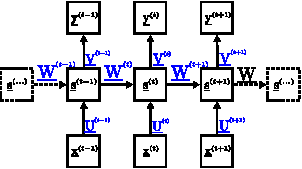
\includegraphics[height=4cm]{img/rnn_unfolded_untie.pdf}
	\end{minipage}
	}
	%~ \iitem{local error terms $\vec \delta^{(t)}$ in backpropagation through time
	\iitem{local error terms in backpropagation through time
		\vspace{1mm}
		%\iitem{for transfer function $f(h) = \tanh(h)$, 
				%i.e.~$f'(h) = \big(1 - f^2(h)\big)$\\
				%%~ and total input $z_i^{(t)} = \smallsum{j=1}{H} W_{ij} h_j^{(t-1)}$
                %}
				}
	%~ \vspace{2mm}
	%$$
		%\delta_i^{(t)} 
		%%quad=\quad \smallfrac{\partial E^T}{\partial h_i^{(t)}}
		%\quad=\quad \smallfrac{\partial y^{(t)}}{\partial z_i^{(t)}}
		%%\quad=\quad \Big(\kern-1.5ex\underbrace{1 - \big(h_i^{(t)}\big)^2
		%\quad=\quad \Big(\kern-1.5ex\underbrace{1 - f^2\big(z_i^{(t)}\big)
				%}_{\begin{array}{c}\\[-4mm]
					%\text{\scriptsize derivative < 1} \\[-1.5mm]
					%\text{\scriptsize i.e.~contracting} 
				%\end{array}} \kern-1.5ex\Big)
			%\cdot \Big(\underbrace{\smallsum{j=1}{H} W_{ij}^\top \delta_j^{(t+1)}
				%}_{\kern-2ex\begin{array}{c}\\[-6mm]
					%\text{\scriptsize potentially} \\[-1.75mm]
					%\text{\scriptsize exploding/vanishing}
				%\end{array}\kern-2ex}\Big)
	%$$
	%~ \vspace{2mm}
	%~ \iitem{over many time steps the local errors $\delta_i^{(t)}$ often vanish}
	\iitem{over many time steps the local errors may also vanish}
		%\vspace{1mm}
		%\iitem{large $\vec w_i \Rightarrow h_i^{(t)} \approx 1 \Rightarrow$ 
		%	derivative $\approx 0$}
		%\iitem{rarely explodes thanks to anti-cyclical derivative $<1$}
	\vspace{2mm}
	\iitem{small short-term errors overshadow large long-term errors}
	%\vspace{2mm}
	%\begin{center}\bf 
	%	How can we learn long time-series without vanishing gradients?
	%\end{center}
\end{frame}

